\section{Generative models}

\subsection{Autoencoders}

Autoencoders map datapoints to latents with an encoder $\bm{\mathcal{E}}$ and latents to their
respective datapoint with a decoder $\bm{\mathcal{D}}$, \[
    \bm{\mathcal{E}}: \mathcal{X} \to \mathcal{Z}, \quad \bm{\mathcal{D}}: \mathcal{Z} \to \mathcal{X}.
\]
We want these to satisfy $\bm{\mathcal{D}}(\bm{\mathcal{E}}(\vec{x})) = \vec{x}$. Generally, the
latent space is smaller than the data space. As a result, new data points can be sampled by sampling
the latent space and using the decoder.

\paragraph{Linear autoencoder.}

The simplest autoencoder is linear, \[
    \bm{\mathcal{E}}(\vec{x}) = \mat{E} \vec{x}, \quad \bm{\mathcal{D}}(\vec{z}) = \mat{D} \vec{z}, \quad \mat{E} \in \R^{m \times d}, \mat{D} \in \R^{d \times m},
\]
where generally $m \ll d$. The reconstruction loss is \[
    \ell[\mat{E}, \mat{D}](\vec{x}) = \frac{1}{2} \| \vec{x} - \hat{\vec{x}} \|^2 = \frac{1}{2} \| (\mat{I} - \mat{D} \mat{E}) \vec{x} \|^2.
\]
It can be shown that the solution to this loss is performing PCA (\textit{\textbf{P}rincipal \textbf{C}omponent 
\textbf{A}nalysis}) on the covariance matrix $\frac{1}{n} \transpose{\mat{X}} \mat{X} \in \R^{d \times d}$
and taking the $m$ principal eigenvectors. The intuition behind this is that we want to retain as
much variance in the data as possible.

\paragraph{Variational autoencoder.}

VAEs (\textit{\textbf{V}ariational \textbf{A}uto\textbf{e}ncoders}) \citep{kingma2013auto} perform
inference by sampling a latent from a prior and decoding it, \[
    \vec{x} = \bm{\mathcal{D}}[\vec{\theta}](\vec{z}), \quad \vec{z} \sim \mathcal{N}(\vec{0}, \mat{I}_m).
\]
However, the question is how to optimize the decoder. In generative modeling, we want to optimize
the likelihood of the data. However, this is not possible for the VAE, so we must bound it using
the ELBO (\textit{\textbf{E}vidence \textbf{L}ower \textbf{Bo}und}),
\begin{align*}
    \log p[\vec{\theta}](\vec{x}) & = \log \int p[\vec{\theta}](\vec{x}, \vec{z}) \mathrm{d}\vec{z} \margintag{Sum rule, where $\vec{z}$ could be anything.}                                                                                                                                                                                                                                                                                                \\
                                  & = \log \int p[\vec{\theta}](\vec{x} \mid \vec{z}) p(\vec{z}) \mathrm{d}\vec{z} \margintag{Product rule. The conditional distribution is induced by the decoder with parameters $\vec{\theta}$.}                                                                                                                                                                                      \\
                                  & = \log \int q(\vec{z}) \lft( p[\vec{\theta}](\vec{x} \mid \vec{z}) \frac{p(\vec{z})}{q(\vec{z})} \rgt) \mathrm{d}\vec{z} \margintag{$q$ can be any distribution over $\vec{z}$, which we will make use of later.}                                                                                                                                                                    \\
                                  & = \log \E_q \lft[ p[\vec{\theta}](\vec{x}\mid \vec{z}) \frac{p(\vec{z})}{q(\vec{z})} \rgt]                                                                                                                                                                                                                                                                                           \\
                                  & \geq \E_q \lft[ \log \lft( p[\vec{\theta}](\vec{x}\mid \vec{z}) \frac{p(\vec{z})}{q(\vec{z})} \rgt) \rgt] \margintag{Jensen's inequality.}                                                                                                                                                                                                                                           \\
                                  & = \E_q \lft[ \log p[\vec{\theta}](\vec{x} \mid \vec{z}) \rgt] - \E_q \lft[ \log \frac{q(\vec{z})}{p(\vec{z})} \rgt]                                                                                                                                                                                                                                                                  \\
                                  & = \E_q \lft[ \log p[\vec{\theta}](\vec{x} \mid \vec{z}) \rgt] - D_{\mathrm{KL}}(q \| p)                                                                                                                                                                                                                                                                                              \\
                                  & = \E_{p[\vec{\vartheta}](\vec{z} \mid \vec{x})} \lft[ \log p[\vec{\theta}](\vec{x} \mid \vec{z}) \rgt] - D_{\mathrm{KL}}(p(\vec{z} \mid \vec{x}) \| p(\vec{z})). \margintag{Since this holds for any distribution over $\vec{z}$, we can replace $q$ by $p[\vec{\vartheta}](\vec{z} \mid \vec{x})$---this distribution is induced by the encoder with parameters $\vec{\vartheta}$.}
\end{align*}
Thus, to maximize the log-likelihood of the data, we maximize the ELBO. The ELBO can be seen as a
reconstruction loss with a regularization term---the KL divergence makes sure that the predicted
distributions over the latent variables stays close to the prior. The advantage of this is that we
get a well-behaving latent space, where the distribution over latents for $\vec{x}$ is an area rather
than a single point. Then, the decoder will see a greater variety of latents during training,
making it perform well on all latents around the prior. As a result, when we want to sample from the
autoencoder, we can sample $\vec{z}$ from the prior and get a good reconstruction
$\vec{x} = \bm{\mathcal{D}}(\vec{z})$. If every training data point instead only had to cover a
single point in the latent space, a sampled latent $\vec{z} \sim p$ would likely not have been seen before by the
decoder and thus give a bad sample.

In general, the posterior $p[\vec{\vartheta}](\vec{z}\mid \vec{x})$ is intractable, so we restrict
it to the Gaussian family of distributions, \[
    \vec{z} \mid \vec{x} \sim \mathcal{N}(\vec{\mu}[\vec{\vartheta}](\vec{x}), \mat{\Sigma}[\vec{\vartheta}](\vec{x}))
\]
Generally, the prior is given as \[
    \vec{z} \sim \mathcal{N}(\vec{0}, \mat{I}).
\]
Consequently, the KL divergence can be computed in closed form, \[
    D_{\mathrm{KL}}(p[\vec{\vartheta}](\vec{z} \mid \vec{x}) \| p) = \frac{1}{2} \lft( \| \vec{\mu}[\vec{\vartheta}](\vec{x}) \|^2 + \tr{\mat{\Sigma}[\vec{\vartheta}](\vec{x})} - \log \det{\mat{\Sigma}[\vec{\vartheta}](\vec{x})}  - m \rgt).
\]
The parameters of the encoder $\vec{\vartheta}$ can be optimized by making use of the
reparameterization trick.

\subsection{Generative adversarial networks}

\begin{marginfigure}
    \centering
    \incfig{adversarial}
    \caption{The loss function of the generator is adversarial in GANs---the generator wants the discriminator to ``think'' that its generations come from ``nature''.}
    \label{fig:adversarial}
\end{marginfigure}

Optimizing the likelihood of the data is not the only way to train a generative model---there are
many ways to provide a training signal to a generative model. In GANs (\textit{\textbf{G}enerative
    \textbf{A}dversarial \textbf{N}etworks}) \citep{goodfellow2020generative}, we introduce a
classifier that distinguishes between samples from ``nature'' and the generator---see
\Cref{fig:adversarial}. The high-level goal of the generator is to ``fool'' the discriminator into
``thinking'' that its generations come from ``nature''. The training signal thus comes from an
adversarial model.

Formally, the discriminator is a binary classifier where 1 means that the sample is real and 0 that
it is not. We have the following augmented distribution over samples and their label, \[
    \tilde{p}(\vec{x}, y) = \frac{1}{2} \lft( y p(\vec{x}) + (1-y)p[\vec{\theta}](\vec{x}) \rgt), \quad y \in \{ 0,1 \},
\]
where $p$ is the true probability distribution and $p[\vec{\theta}]$ denotes the model's implicit
distribution over samples. The theoretical Bayes-optimal classifier is \[
    \mathbb{P}(y = 1 \mid \vec{x}) = \frac{\mathbb{P}(\vec{x} \mid y = 1) \mathbb{P}(y = 1)}{\mathbb{P}(\vec{x})} = \frac{p(\vec{x})}{p(\vec{x}) + p[\vec{\theta}](\vec{x})}. \margintag{Assume a 1-to-1 ratio of samples, so the prior is $\nicefrac{1}{2}$.}
\]
We can then train the generator to minimize the logistic log-likelihood of the Bayes-optimal
discriminator,
\begin{align*}
    \ell^\star(\vec{\theta}) & = \E_{\vec{x}, y \sim \tilde{p}} \lft[ y \log \mathbb{P}(y=1 \mid \vec{x}) + (1-y) \log (1-\mathbb{P}(y=1 \mid \vec{x})) \rgt]                                                                                                                                                                              \\
                       & = \E_{\vec{x}, y \sim \tilde{p}} \lft[ y \log \frac{p(\vec{x})}{p(\vec{x}) + p[\vec{\theta}](\vec{x})} + (1-y) \log \frac{p[\vec{\theta}](\vec{x})}{p(\vec{x}) + p[\vec{\theta}](\vec{x})} \rgt]                                                                                                            \\
                       & = \E_p \lft[ \log \frac{p(\vec{x})}{p(\vec{x}) + p[\vec{\theta}](\vec{x})} \rgt] + \E_{p[\vec{\theta}]} \lft[ \log \frac{p[\vec{\theta}](\vec{x})}{p(\vec{x}) + p[\vec{\theta}](\vec{x})} \rgt]                                                                                                             \\
                       & = \E_p \lft[ \log p(\vec{x}) \rgt] - \E_p \lft[ \log \lft( p(\vec{x}) + p[\vec{\theta}](\vec{x}) \rgt) \rgt]                                                                                                                                                                                                \\
                       & \quad + \E_{p[\vec{\theta}]} \lft[ \log p[\vec{\theta}](\vec{x}) \rgt] - \E_{p[\vec{\theta}]} \lft[ \log \lft( p(\vec{x}) + p[\vec{\theta}](\vec{x}) \rgt) \rgt]                                                                                                                                            \\
                       & = -\frac{1}{2} H(p) -\frac{1}{2} H(p[\vec{\theta}]) + H\lft(\frac{1}{2} (p + p[\vec{\theta}])\rgt) - \log 2 \margintag{Combine the two negative terms into an expectation \wrt $\tilde{p}$. Then, get the argument of the logarithm to be $\tilde{p}$ to get the entropy term of $\tilde{p} = \frac{1}{2} (p + p[\vec{\theta}])$.} \\
                       & = D_{\mathrm{JS}}(p \| p[\vec{\theta}]) - \log 2.
\end{align*}
In conclusion, minimizing the logistic log-likelihood of the optimal classifier leads to a loss
function that is the discrepancy between the nature distribution and the model distribution.

Generally, the Bayes-optimal classifier is intractable. Instead, we parameterize a discriminator, \[
    q[\vec{\varphi}]: \mathcal{X} \to [0,1], \quad \vec{\varphi} \sim \Phi.
\]
Since this model cannot be better than the Bayes-optimal classifier, we have the following bound, \[
    \ell^\star(\vec{\theta}) \geq \sup_{\vec{\varphi} \in \Phi} \ell(\vec{\theta}, \vec{\varphi}),
\]
where \[
    \ell(\vec{\theta}, \vec{\varphi}) \doteq \E_{\tilde{p}} \lft[ y \log q[\vec{\varphi}](\vec{x}) + (1-y) \log (1-q[\vec{\varphi}](\vec{x})) \rgt].
\]

\begin{marginfigure}
    \centering
    \incfig{extragradient}
    \caption{Illustration of the extragradient algorithm for updating $\vec{\theta}$.}
    \label{fig:extragradient}
\end{marginfigure}

In practice, we thus first optimize the discriminator and then the generator, \[
    \vec{\theta}^\star, \vec{\varphi}^\star \in \argmin_{\vec{\theta} \in \Theta} \argmax_{\vec{\varphi} \in \Phi} \ell(\vec{\theta}, \vec{\varphi}).
\]
This can also be interpreted as a two-player zero-sum game---we need the extragradient optimization algorithm,
\begin{align*}
    \vec{\theta}_{t+1} & = \vec{\theta}_t - \eta \grad{\ell(\vec{\theta}_{t+\nicefrac{1}{2}}, \vec{\varphi}_t)}{\vec{\theta}}, \quad \vec{\theta}_{t+\nicefrac{1}{2}} \doteq \vec{\theta}_t - \eta \grad{\ell(\vec{\theta}_t, \vec{\varphi}_t)}{\vec{\theta}} \\
    \vec{\varphi}_{t+1} & = \vec{\varphi}_t + \eta \grad{\ell(\vec{\theta}_t, \vec{\varphi}_{t+\nicefrac{1}{2}})}{\vec{\varphi}}, \quad \vec{\varphi}_{t+\nicefrac{1}{2}} \doteq \vec{\varphi}_t + \eta \grad{\ell(\vec{\theta}_t, \vec{\varphi}_t)}{\vec{\varphi}}.
\end{align*}
This is necessary, because alternating gradient descent/ascent is not guaranteed to converge to local optima.

In practice, it is also necessary to set the loss function of the generator to be the following, \[
    \ell(\vec{\theta} \mid \vec{\varphi}) = \E_{p[\vec{\theta}]} \lft[ -\log q[\vec{\varphi}](\vec{x}) \rgt]. \margintag{Initially, it was $\E_{p[\vec{\theta}]} \lft[ \log(1-q_{\vec{\varphi}}(\vec{x})) \rgt]$.}
\]
As a result, the generator does not saturate when its performance is poor, because the gradient is
bounded as $q_{\vec{\varphi}}(\vec{x}) \to 1$.

\subsection{Diffusion models}

As in VAEs, we want to map a simple distribution to a target distribution over the data, \[
    \pi \mapsto p[\vec{\theta}] \approx p,
\]
where $\pi$ is the simple distribution. Whereas VAEs do this in a single pass, diffusion models do it incrementally, \[
    \pi = \pi_T \mapsto \pi_{T-1} \mapsto \cdots \mapsto \pi_0 \approx p.
\]

\paragraph{Stochastic differential equation view.}

One can view the diffusion process in a continuous time by an SDE (\textit{\textbf{S}tochastic
\textbf{D}ifferential \textbf{E}quation}) \citep{song2019generative,song2020score}, \[
    \mathrm{d}\vec{x}_t = -\frac{1}{2} \beta_t \vec{x}_t \mathrm{d}t + \sqrt{\beta_t} \mathrm{d}\mathbb{W}_t,
\]
where $\mathrm{d}\mathbb{W}_t$ is a Wiener process.\sidenote{The Wiener process $\mathrm{d}\mathbb{W}_t$ is a Gaussian distribution with variance $\mathrm{d}t$.} The time-reversed SDE can be computed by the following, \[
    \mathrm{d}\vec{x}_t = \lft( -\frac{1}{2} \beta_t \vec{x}_t - \beta_t \grad{\log q_t(\vec{x}_t)}{\vec{x}_t} \rgt) \mathrm{d}t + \sqrt{\beta_t} \mathrm{d} \tilde{\mathbb{W}}_t,
\]
where $\mathrm{d}\tilde{\mathbb{W}}_t$ is the reversed Wiener process. Intuitively, denoising amounts to
approximating a vector field over the gradient of the probability distribution---moving towards areas
with high probability density. Effectively, we are performing gradient ascent on the log-probability
perturbed by a Wiener noise process. Hence, we can think of diffusion models as approximating the
score function $\grad{\log p(\vec{x})}{}$.

\begin{figure}[h]
    \centering
    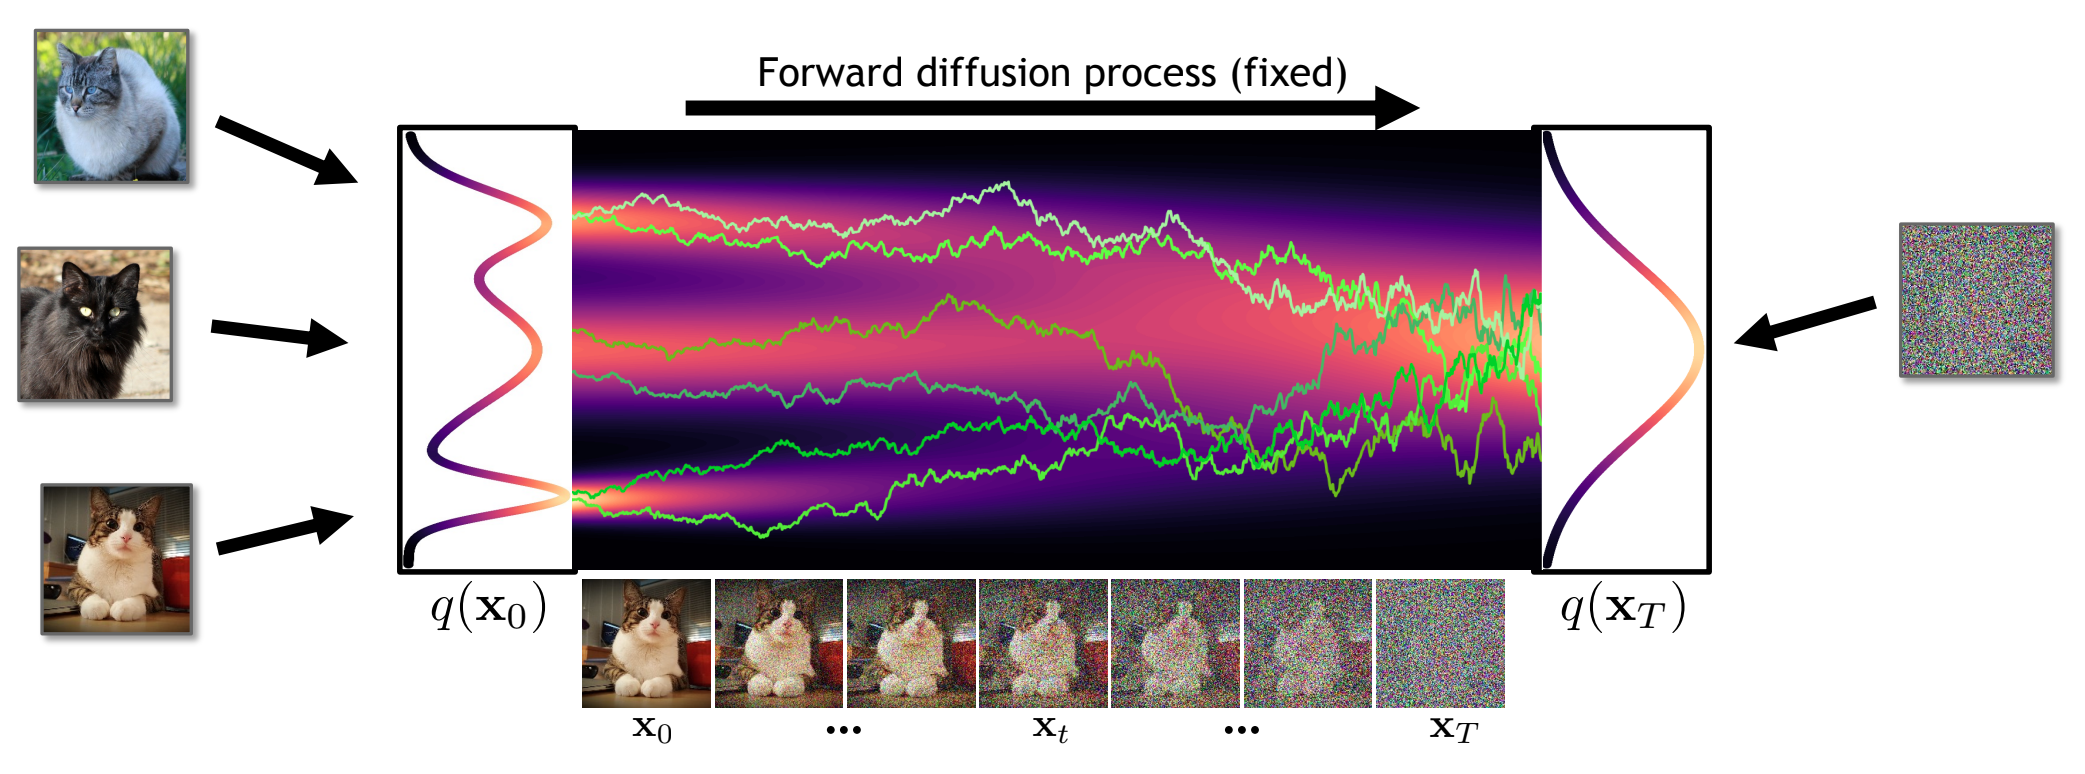
\includegraphics[width=\textwidth]{figures/sde}
    \caption{Diffusion models through the lens of SDEs \citep{song2020score}.}
    \label{fig:sde}
\end{figure}

\paragraph{Evidence lower bound view.}

One can also present diffusion models in a less involved way by deriving an ELBO. Let the following be the forward process, \[
    \vec{x}_t = \sqrt{1-\beta_t} \vec{x}_{t-1} + \sqrt{\beta}_t \vec{\epsilon}_t, \quad \vec{\epsilon}_t \sim \mathcal{N}(\vec{0}, \mat{I}).
\]
Note that the energy of the stochastic process evolves as follows, \[
    \E \lft[ \| \vec{x}_t \|^2 \;\middle|\; \vec{x}_{t-1} \rgt] = (1-\beta_t) \| \vec{x}_{t-1} \|^2 + \beta_t \tr{\mat{I}}.
\]
Fixing the scale of the data such that $\E \lft[ \| \vec{x}_0 \|^2 \rgt] = \tr{\mat{I}} =
\mathrm{dim}(\vec{x}_0)$ results in energy conservation.

Let $q$ be the kernel of the forward diffusion Markov chain and $p[\vec{\theta}]$ the learned kernel
for the time-reversed one. Furthermore, let $p$ be the actual distribution over data points. Then,
the log-likelihood of a sample $\vec{x}_0 \sim p$ can be lower bounded as follows,
\begin{align*}
    \log p[\vec{\theta}](\vec{x}_0) & = \log \int p[\vec{\theta}](\vec{x}_{0:T}) \mathrm{d}\vec{x}_{1:T} \margintag{Sum rule.} \\
                                    & = \log \int q(\vec{x}_{1:T} \mid \vec{x}_0) \frac{p[\vec{\theta}](\vec{x}_{0:T})}{q(\vec{x}_{1:T} \mid \vec{x}_0)} \mathrm{d}\vec{x}_{1:T} \\
                                    & \geq \E_{q(\vec{x}_{1:T} \mid \vec{x}_0)} \lft[ \log \frac{p[\vec{\theta}](\vec{x}_{0:T})}{q(\vec{x}_{1:T} \mid \vec{x}_0)} \rgt] \margintag{Jensen's inequality.} \\
                                    & = \E_{q(\vec{x}_{1:T} \mid \vec{x}_0)} \lft[ \sum_{t=0}^{T} \log p[\vec{\theta}](\vec{x}_t \mid \vec{x}_{t+1:T}) - \sum_{t=1}^{T} \log q(\vec{x}_t \mid  \vec{x}_0, \vec{x}_{1:t-1}) \rgt] \margintag{Product rule.} \\
                                    & = \E_{q(\vec{x}_{1:T} \mid \vec{x}_0)} \lft[ \sum_{t=0}^{T} \log p[\vec{\theta}](\vec{x}_t \mid \vec{x}_{t+1}) - \sum_{t=1}^{T} \log q(\vec{x}_t \mid \vec{x}_0, \vec{x}_{t-1}) \rgt] \margintag{Markov property.} \\
                                    & = \E_{q(\vec{x}_{1:T} \mid \vec{x}_0)} \Biggl[ \log p[\vec{\theta}](\vec{x}_0 \mid \vec{x}_1) + \log \frac{p(\vec{x}_T)}{q(\vec{x}_T \mid \vec{x}_0)} \\
                                    & \quad \quad + \sum_{t=1}^{T-1} \log \frac{p[\vec{\theta}](\vec{x}_t \mid \vec{x}_{t+1})}{q(\vec{x}_t \mid \vec{x}_0, \vec{x}_{t-1})} \Biggr] \\
                                    & = \E_q \lft[ \log p[\vec{\theta}](\vec{x}_0 \mid \vec{x}_1) \rgt] + \sum_{t=1}^{T-1} \E_q \lft[ \log \frac{p[\vec{\theta}](\vec{x}_t \mid \vec{x}_{t+1})}{q(\vec{x}_t \mid \vec{x}_0, \vec{x}_{t-1})} \rgt] \\
                                    & \quad \quad + \E_q \lft[ \log \frac{p(\vec{x}_T)}{q(\vec{x}_T \mid \vec{x}_0)} \rgt] \\
                                    & = \E_q \lft[ \log p[\vec{\theta}](\vec{x}_0 \mid \vec{x}_1) \rgt] - \sum_{t=1}^{T-1} D_{\mathrm{KL}}(q(\vec{x}_t \mid \vec{x}_{t-1}, \vec{x}_0) \| p[\vec{\theta}](\vec{x}_t \mid \vec{x}_{t+1})) \\
                                    & \quad \quad - D_{\mathrm{KL}}(q(\vec{x}_T \mid \vec{x}_0) \mid \pi).
\end{align*}
We can divide this up into loss terms (that we want to maximize) per timestep, \[
    \ell_t = \begin{cases}
        \E_q \lft[ \log p[\vec{\theta}](\vec{x}_0 \mid \vec{x}_1) \rgt] & t = 0 \\
        -D_{\mathrm{KL}}(q(\vec{x}_t \mid \vec{x}_{t-1}, \vec{x}_0) \| p[\vec{\theta}](\vec{x}_t \mid \vec{x}_{t+1})) & 0 < t < T \\
        -D_{\mathrm{KL}}(q(\vec{x}_T \mid \vec{x}_0) \mid \pi) & t = T.
    \end{cases}
\]
Here, the KL divergences can analytically be computed, because all $q$ are Gaussians and if the steps
$\beta_t$ are small enough, the reverse distributions $p[\vec{\theta}]$ can be accurately approximated by
Gaussians---this is generally how they are parameterized, \[
    \vec{x}_{t-1} \mid \vec{x}_t \sim \mathcal{N}(\vec{\mu}[\vec{\theta}](\vec{x}_t, t), \mat{\Sigma}[\vec{\theta}](\vec{x}_t, t)).
\]
Often, the covariance matrix is fixed and only the mean is predicted.

\paragraph{Entropy bounds.}

Using conditional entropy, we can derive the following, \[
    H(\vec{x}_{t-1} \mid \vec{x}_t) = H(\vec{x}_t \mid \vec{x}_{t-1}) + H(\vec{x}_{t-1}) - H(\vec{x}_t).
\]
Since the unit distribution is the maximum entropy distribution, we have the following entropy bounds between timesteps, \[
    H(\vec{x}_{t-1} \mid \vec{x}_t) \leq H(\vec{x}_t \mid \vec{x}_{t-1}).
\]
As such, the entropy of the reverse process is bounded by the entropy of the forward process.

\paragraph{Simplified model.}

Consider a noise schedule $\{ \beta_t \}_{t=1}^T$ and define \[
    \bar{\alpha}_t \doteq \prod_{\tau=1}^{t} (1-\beta_\tau), \quad \bar{\beta}_t \doteq 1 - \bar{\alpha}_t.
\]
Using these, we can compute the forward process in closed form at any timestep, \[
    \vec{x}_t \sim \mathcal{N}(\sqrt{\bar{\alpha}_t} \vec{x}_0, \bar{\beta}_t \mat{I}).
\]
Furthermore, the $q$ targets in the ELBO can be derived to be the following, \[
    \vec{x}_{t-1} \mid \vec{x}_t, \vec{x}_0 \sim \mathcal{N}(\vec{\mu}(\vec{x}_t, \vec{x}_0, t), \tilde{\beta}_t \mat{I}).
\]
where \[
    \vec{\mu}(\vec{x}_t, \vec{x}_0, t) \doteq \frac{\sqrt{\bar{\alpha}_{t-1}} \beta_t}{1- \bar{\alpha}_t} \vec{x}_0 + \frac{1-\bar{\alpha}_{t-1}}{1-\bar{\alpha}_t} \sqrt{1-\beta_t} \vec{x}_t, \quad \tilde{\beta}_t \doteq \frac{1-\bar{\alpha}_{t-1}}{1-\bar{\alpha}_t} \beta_t.
\]
Now, the divergences for $0 < t < T$ in the ELBO simplify to \[
    \ell_t = -\frac{1}{2 \sigma_t^2} \| \vec{\mu}(\vec{x}_t, \vec{x}_0, t) - \vec{\mu}[\vec{\theta}](\vec{x}_t, t) \|^2,
\]
where $\sigma_t^2 \in [\beta_t, \tilde{\beta}_t]$ is the chosen fixed variance of the backward process.

We can also use a different definition of $\vec{\mu}(\vec{x}_t, \vec{x}_0, t)$ by noting the forward process, \[
    \vec{x}_t = \sqrt{\bar{\alpha}_t} \vec{x}_0 + \sqrt{1-\bar{\alpha}_t} \vec{\epsilon}, \quad \vec{\epsilon} \sim \mathcal{N}(\vec{0}, \mat{I}) \\
\]
Rewriting yields \[
    \vec{x}_0 = \frac{1}{\sqrt{\bar{\alpha}_t}} \vec{x}_t - \frac{\sqrt{1-\bar{\alpha}_t}}{\sqrt{\bar{\alpha}_t}} \vec{\epsilon}.
\]
As such, we can write $\vec{\mu}(\vec{x}_t, \vec{x}_0, t)$ as \[
    \vec{\mu}(\vec{x}_t, \vec{x}_0, t) = \frac{1}{\sqrt{\alpha_t}} \lft( \vec{x}_t - \frac{\beta_t}{\sqrt{1-\bar{\alpha}_t}} \vec{\epsilon} \rgt).
\]
Note that $\vec{\epsilon}$ fully determines $\vec{x}_t$ and $\vec{x}_0$ is constant. Hence, the backward process actually only needs to predict $\vec{\epsilon}$ by a network $\vec{\epsilon}[\vec{\theta}](\vec{x}_t, t)$. Using this observation a new loss function can be derived, \[
    \E_q [\mathcal{L}_t \mid \vec{x}_0] = \E_{\vec{\epsilon}} \lft[\lambda(t) \| \vec{\epsilon} - \vec{\epsilon}[\vec{\theta}](\vec{x}_t, t) \|^2 \rgt], \quad \lambda(t) \doteq \frac{\beta_t^2}{2 \sigma_t^2 \alpha_t (1-\bar{\alpha}_t)}.
\]
In practice, the full loss is often approximated by \[
    \ell(\vec{\theta} \mid \vec{x}_0) = \frac{1}{T} \sum_{t=1}^{T} \E_{\vec{\epsilon}} \lft[ \| \vec{\epsilon} - \vec{\epsilon}[\vec{\theta}](\vec{x}_t, t) \|^2 \;\middle|\; \vec{x}_0 \rgt].
\]
We make a Monte Carlo approximation of this loss by uniformly sampling a timestep $t$ and sampling noise $\vec{\epsilon} \sim \mathcal{N}(\vec{0}, \mat{I})$.
